\documentclass[../Head/Main.tex]{subfiles}
\begin{document}
	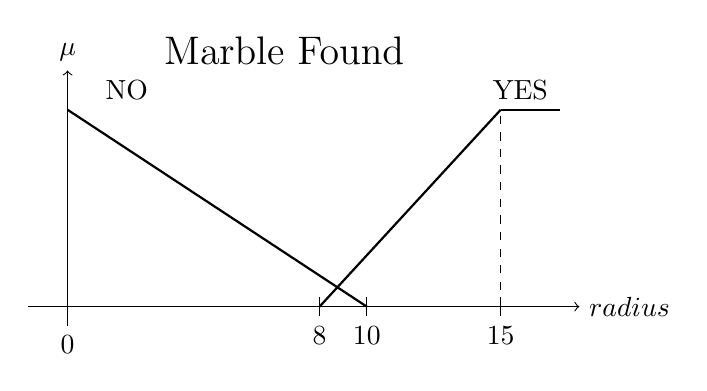
\begin{tikzpicture}
		\draw [->](0,-0.25)--(0,3) node[anchor = south]
			{$\mu$};
		\draw [->](-0.5,0)--(6.5,0) node[right]{$radius$};
		\node[anchor = north] at (0,-0.25) {$0$};
		
		\node at (2.75,3.25) {\Large Marble Found};
		\node at (0.75,2.75) {NO};
		\node at (5.75,2.75) {YES};
			
		\draw (5.5,0.125) -- (5.5,-0.125)
			node[anchor = north] {$15$};
		\draw[dashed] (5.5,0) -- (5.5,2.5);
		
		\draw (3.2,0.125) -- (3.2,-0.125)
			node[anchor = north] {$8$};
			
		\draw (3.8,0.125) -- (3.8,-0.125)
			node[anchor = north] {$10$};	
		
		\draw[thick] (5.5,2.5) -- (6.25,2.5);
		
		\draw[thick] (0,2.5) -- (3.8,0);
		\draw[thick] (5.5,2.5) -- (3.2,0);		
	\end{tikzpicture}
\end{document}